\section{Persistent Homology of a RingCT}

We will be using homology and persistent homology in multiple ways, the implementation and interpretation may differ between cases.  In particular we will be using a \textit{Vietoris-Rips Complex} to define the persistent homology for the RingCT case (where height is the filtration parameter) and a `Flagser' method for the connectivity of the graph case.  We will go into some detail showing the persistence diagram for a ring, which is the simplest case available as our metric space is 1 dimension (the block height).  

The main idea of TDA is that of \textit{persistence};  a sub-complex of a simplicial complex is constructed by providing a parameter and watching how that sub-complex changes from sub-complexes to the full simplicial complex as the parameter is swept.  In our context, the transactions composing the ring are the vertices, the parameter being swept is the block height, and a vertex is joined with another vertex if its distance is within that height of the vertex.  Persistent Homology uses the Union Find algorithm to find unions.  In \ref{UnionFind} we show which set each transaction in a ring is a member of as the algorithm progresses.  Each vertex begins as the singleton set containing just that vertex

In practice we will simply call \textit{Giotto's} Vietoris-Rips functionality and output a persistence diagram.  Indeed this occurs when the \textit{MoneroAna.tx} object is instantiated.  We expect these block height persistence diagrams to be used in a multitude of ways.  
\begin{itemize}
\item Unsupervised Machine Learning; the diagrams themselves occupy a metric space and can be used for clustering (bottle neck distances, Wasserstein distances, Frechet mean)
\item Supervised Machine Learning; the decoy algorithm is implemented at the wallet level, not the protocol level, as such multiple decoy models exist in the wild.  An experiment could be to generate transactions from a variety of wallets and develop a model to predict which wallet a signer of some transaction is using.  In the context of EAE attacks, an exchange can potentially ascertain the external wallet used by a customer.
\item Search optimization.  This is my current focus and most relevant for the context of EAE.  The intersection of taint trees can potentially be searched rather quickly by careful considerations of these diagrams.  Say an exchange is looking for potential common transactions in the histories of two transactions.  If the two transactions are the same then so too is the block height and so are the block ranges to all orders or persistence.  Regions where the diagrams do not overlap can at least be temporarily ignored while regions of overlap are searched.  I am looking for conditions (or reasons why they do not exist) in which the taint trees can be pruned and intersections can be found in potentially log(number of paths).
\item Establishing Anonymity Sets/Confusion Matrices.

\end{itemize}

\subsection{Worked example}

For a given RingCT we'd like to be able to evaluate the likelihood subrings came from a decoy selection algorithm, find similar and comparable rings.  
We can also develop summary statistics about the nature of these rings and representations appropriate for Machine Learning.   

\begin{figure}[h]
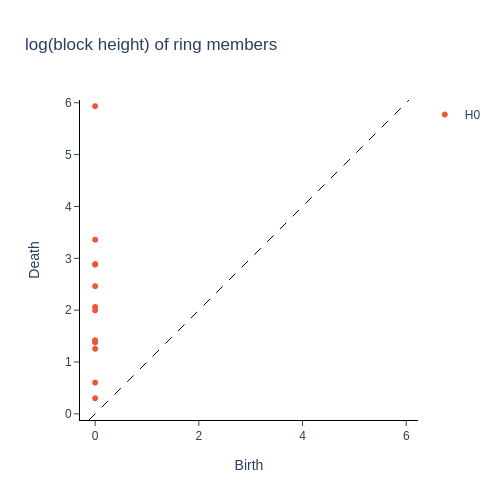
\includegraphics[scale=0.5]{block_height}
\caption{Persistence diagram showing the birth-death pairs of a single ring.  A log scale is shown to separate the points on the graph.  A persistence diagram is a concise representation of all the information shown in Tables \ref{tab:pers2}, \ref{tab:pers}, \ref{UnionFind}.  These diagrams can be analyzed in bulk to find means, anomalies, a basis for Machine Learning and More!}
\label{fig:alpha}
\end{figure}

\begin{center}
\begin{table}
\begin{tabular}{|c|c|c|}

\hline
 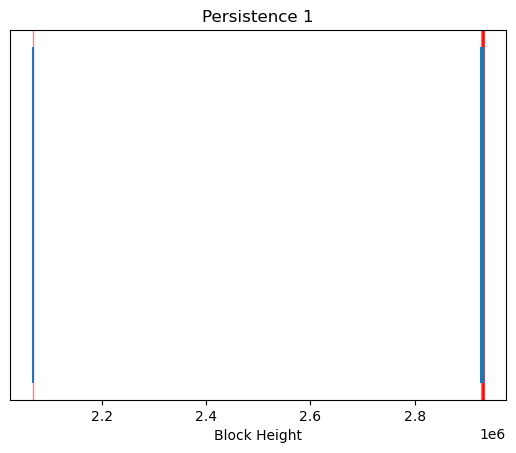
\includegraphics[scale=0.3]{Pers2_00} & 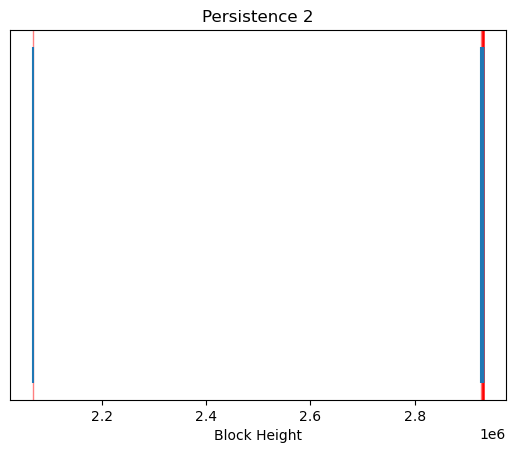
\includegraphics[scale=0.3]{Pers2_01} & 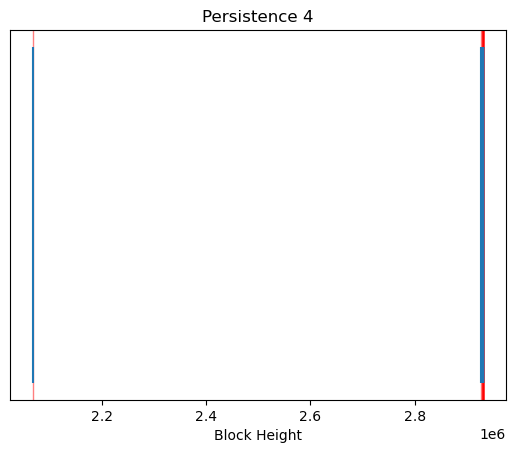
\includegraphics[scale=0.3]{Pers2_02} \\ \hline
  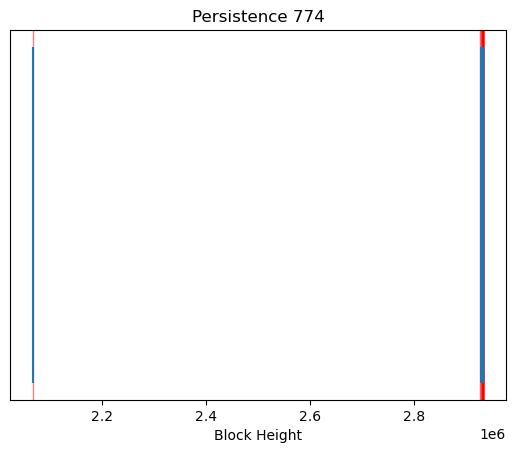
\includegraphics[scale=0.3]{Pers2_12} & 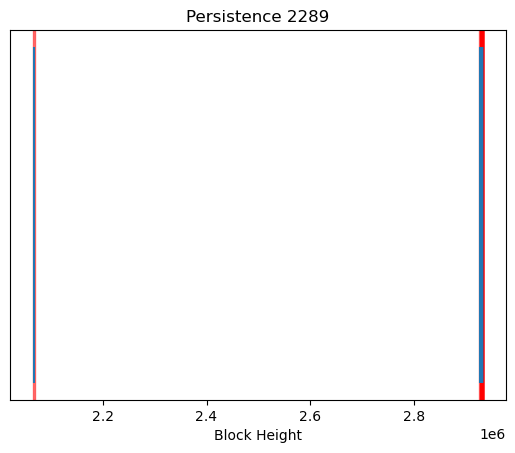
\includegraphics[scale=0.3]{Pers2_13} & 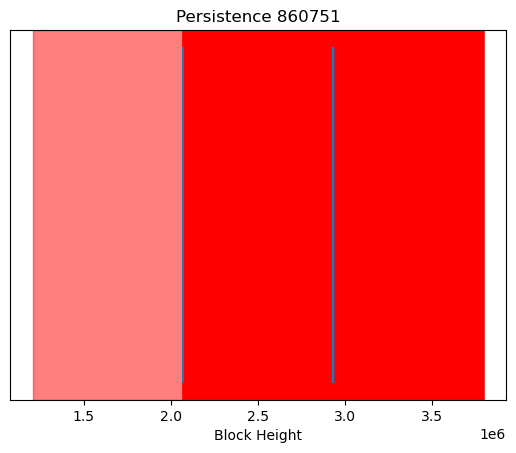
\includegraphics[scale=0.3]{Pers2_14} \\ \hline
\end{tabular}
\caption{As the filtration progresses, holes are filled, joining neighboring transactions into a larger simplex.  Only the first three and last three steps of the algorithm are shown, all of the structure during the intermediate heights is confined to the band on the right side, shown in greater detail in the next diagram. 
In this particular ring, one of the transactions is far older than the others, requiring a large parameter for the height to join the tx with the other transactions.}
\label{tab:pers2}
\end{table}
\end{center}

\begin{center}
\begin{table}
\begin{tabular}{|c|c|c|}
\hline
 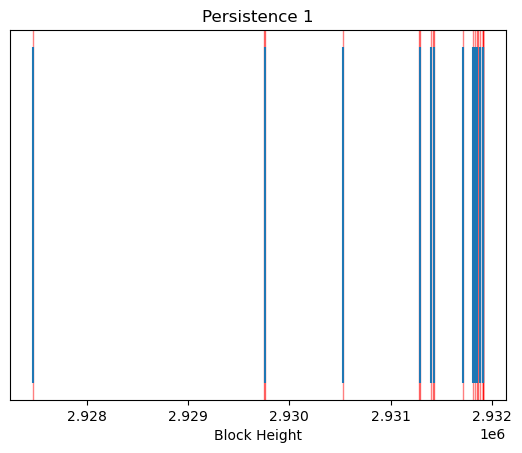
\includegraphics[scale=0.3]{Pers_00} & 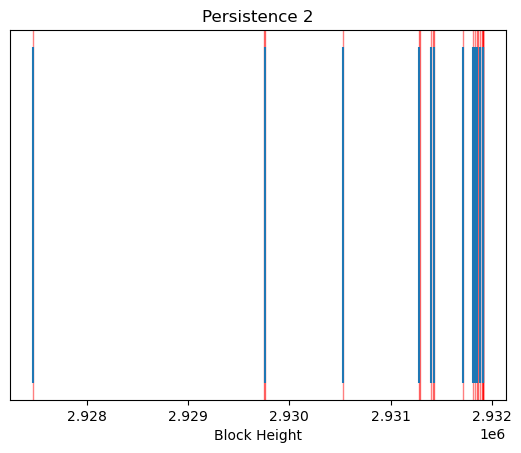
\includegraphics[scale=0.3]{Pers_01} & 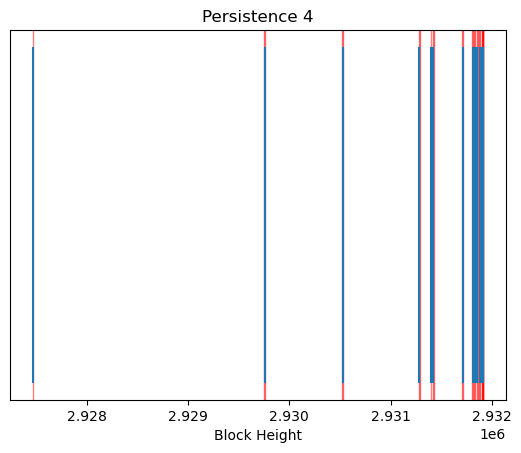
\includegraphics[scale=0.3]{Pers_02} \\ \hline
  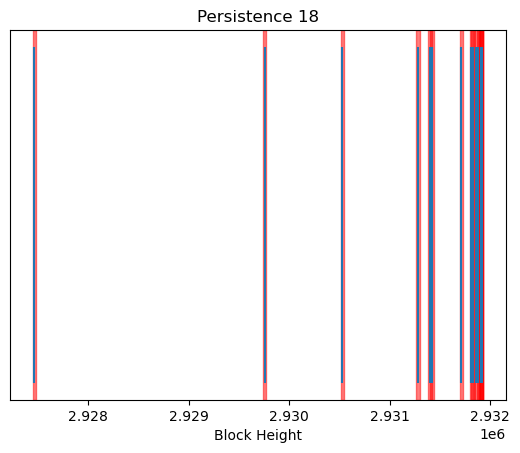
\includegraphics[scale=0.3]{Pers_03} & 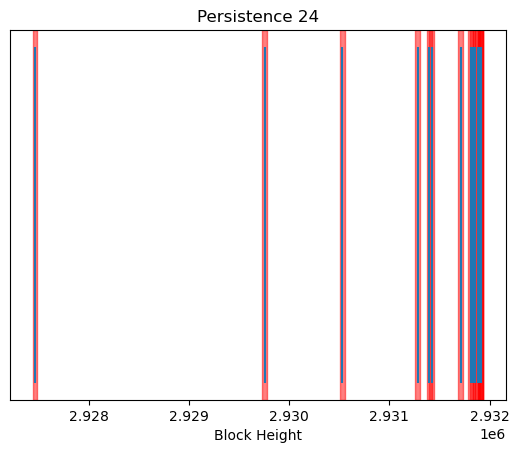
\includegraphics[scale=0.3]{Pers_04} & 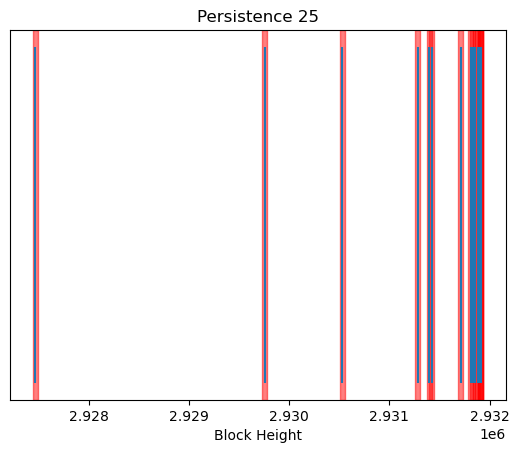
\includegraphics[scale=0.3]{Pers_05} \\ \hline
 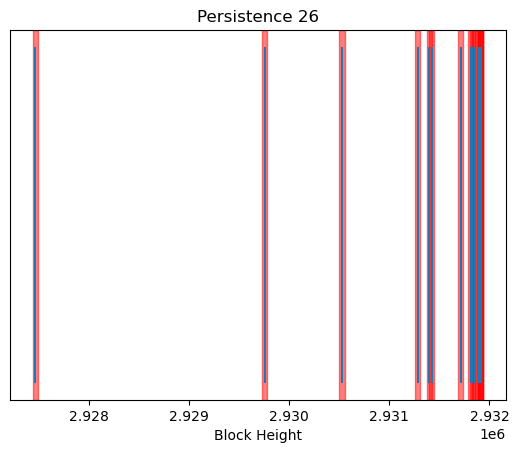
\includegraphics[scale=0.3]{Pers_06} & 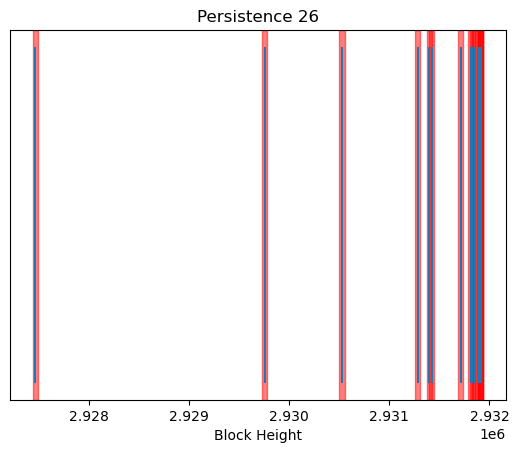
\includegraphics[scale=0.3]{Pers_07} & 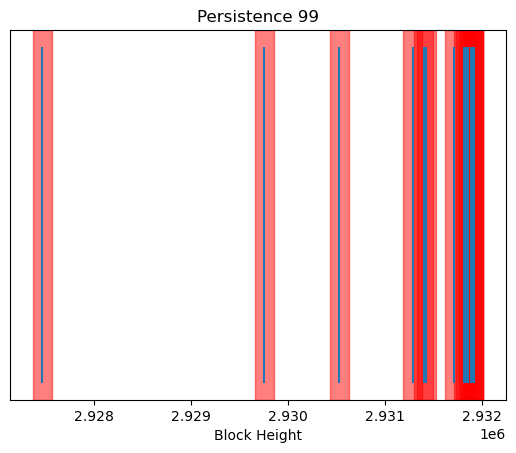
\includegraphics[scale=0.3]{Pers_08} \\ \hline
 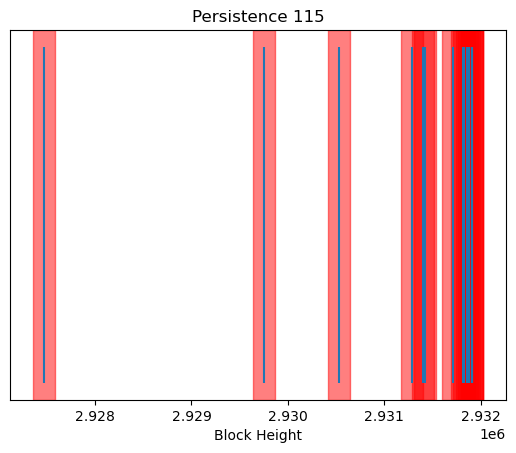
\includegraphics[scale=0.3]{Pers_09} & 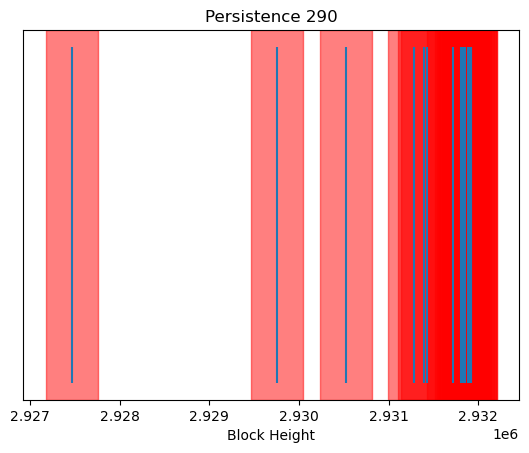
\includegraphics[scale=0.3]{Pers_10} & 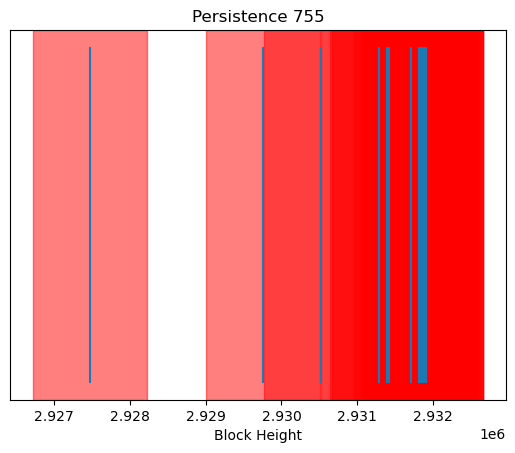
\includegraphics[scale=0.3]{Pers_11} \\ \hline
  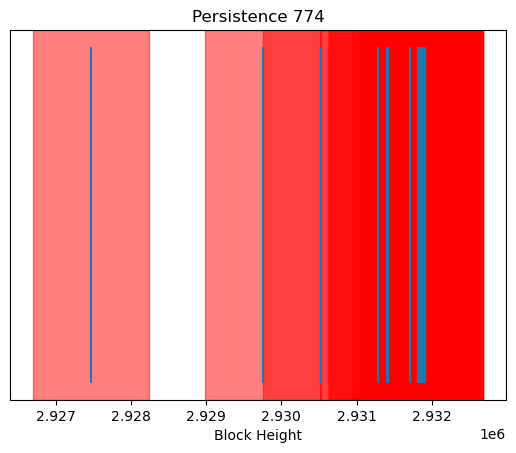
\includegraphics[scale=0.3]{Pers_12} & 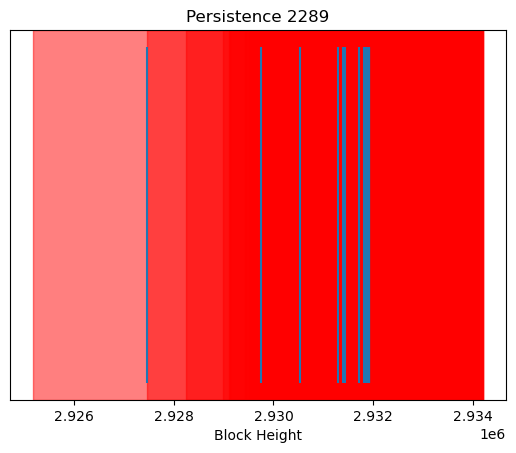
\includegraphics[scale=0.3]{Pers_13} & 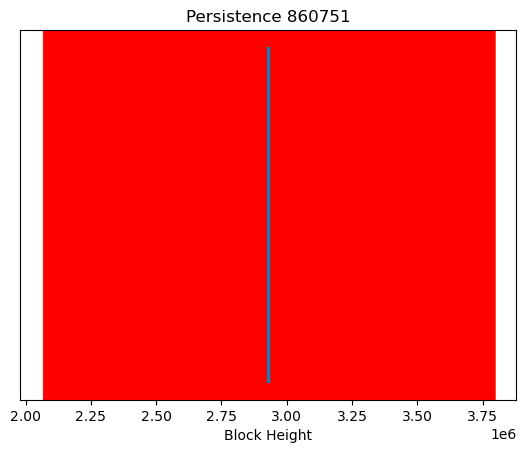
\includegraphics[scale=0.3]{Pers_14} \\ \hline
\end{tabular}
\caption{
As the filtration progresses, holes are filled, joining neighboring transactions into a larger simplex.  The fine structure at the different orders of the filtration are evident as we have zoomed into just the right side of the previous diagram.}
\label{tab:pers}
\end{table}
\end{center}


\begin{center}
\begin{sidewaystable}
\scalebox{0.9}{
\begin{tabular}{|c|c|c|c|c|c|c|c|c|c|c|c|c|c|c|c|c|} 
\hline
block height  & 2066715 & 2927466 & 2929755 & 2930529 & 2931284 & 2931399 & 2931423 & 2931713 & 2931812 & 2931830 & 2931856 & 2931881 & 2931907 & 2931909 & 2931913 & 2931914 \\
\hline \hline
iter 0  & 0 & 1 & 2 & 3 & 4 & 5 & 6 & 7 & 8 & 9 & 10 & 11 & 12 & 13 & 14 & 15 \\ \hline
iter 1  & 0 & 1 & 2 & 3 & 4 & 5 & 6 & 7 & 8 & 9 & 10 & 11 & 12 & 13 & 14 & 14 \\ \hline
iter 2  & 0 & 1 & 2 & 3 & 4 & 5 & 6 & 7 & 8 & 9 & 10 & 11 & 12 & 12 & 14 & 14 \\ \hline
iter 3*  & 0 & 1 & 2 & 3 & 4 & 5 & 6 & 7 & 8 & 9 & 10 & 11 & 12 & 12 & 14 & 14 \\ \hline
iter 4  & 0 & 1 & 2 & 3 & 4 & 5 & 6 & 7 & 8 & 8 & 10 & 11 & 12 & 12 & 12 & 12 \\ \hline
iter 5  & 0 & 1 & 2 & 3 & 4 & 5 & 5 & 7 & 8 & 8 & 10 & 11 & 12 & 12 & 12 & 12 \\ \hline
iter 6  & 0 & 1 & 2 & 3 & 4 & 5 & 5 & 7 & 8 & 8 & 10 & 10 & 12 & 12 & 12 & 12 \\ \hline
iter 7  & 0 & 1 & 2 & 3 & 4 & 5 & 5 & 7 & 8 & 8 & 10 & 10 & 12 & 12 & 12 & 12 \\ \hline
iter 8  & 0 & 1 & 2 & 3 & 4 & 5 & 5 & 7 & 8 & 8 & 10 & 10 & 12 & 12 & 12 & 12 \\ \hline
iter 9  & 0 & 1 & 2 & 3 & 4 & 5 & 5 & 7 & 7 & 7 & 10 & 10 & 10 & 10 & 10 & 10 \\ \hline
iter 10  & 0 & 1 & 2 & 3 & 4 & 4 & 4 & 7 & 7 & 7 & 10 & 10 & 10 & 10 & 10 & 10 \\ \hline
iter 11  & 0 & 1 & 2 & 3 & 4 & 4 & 4 & 7 & 7 & 7 & 7 & 7 & 7 & 7 & 7 & 7 \\ \hline
iter 12  & 0 & 1 & 2 & 3 & 3 & 3 & 3 & 7 & 7 & 7 & 7 & 7 & 7 & 7 & 7 & 7 \\ \hline
iter 13  & 0 & 1 & 2 & 2 & 2 & 2 & 2 & 7 & 7 & 7 & 7 & 7 & 7 & 7 & 7 & 7 \\ \hline
iter 14  & 0 & 1 & 1 & 1 & 1 & 1 & 1 & 7 & 7 & 7 & 7 & 7 & 7 & 7 & 7 & 7 \\ \hline
iter 15  & 0 & 0 & 0 & 0 & 0 & 0 & 0 & 7 & 7 & 7 & 7 & 7 & 7 & 7 & 7 & 7 \\ \hline
iter 16  & 0 & 0 & 0 & 0 & 0 & 0 & 0 & 0 & 0 & 0 & 0 & 0 & 0 & 0 & 0 & 0 \\ \hline
\end{tabular}}
\begin{center}
\caption{\label{UnionFind} Persistent Homology uses the Union Find algorithm to find unions.  Here we show which set each transaction in a ring is a member of as the algorithm progresses.}
\end{center}
\end{sidewaystable}
\end{center}
